\documentclass[a4paper,12pt]{article}

\author{\textbf{Софиа Белен Лопес Висенс}\\Группа Б02-903\\ \large Московский физико-технический институт}
\title{\textbf{Задание 1}\\Молекурялная динамика}
\date{}

\usepackage[margin=0.9in]{geometry}
\usepackage{graphicx}
\usepackage{float}
\usepackage[utf8]{inputenc}
\usepackage[T2A]{fontenc}
\usepackage{textcomp}
\usepackage{amsmath, amssymb}
\usepackage{siunitx}
\usepackage{subcaption}
\usepackage{multirow}

\renewcommand{\figurename}{Рис.}
\renewcommand{\tablename}{Таблица}
\renewcommand*\contentsname{Содержание}

\begin{document}
\maketitle
\newpage
\tableofcontents
\newpage

\section{Время установления распределения Максвелла}

\begin{figure}[H]
    \centering
    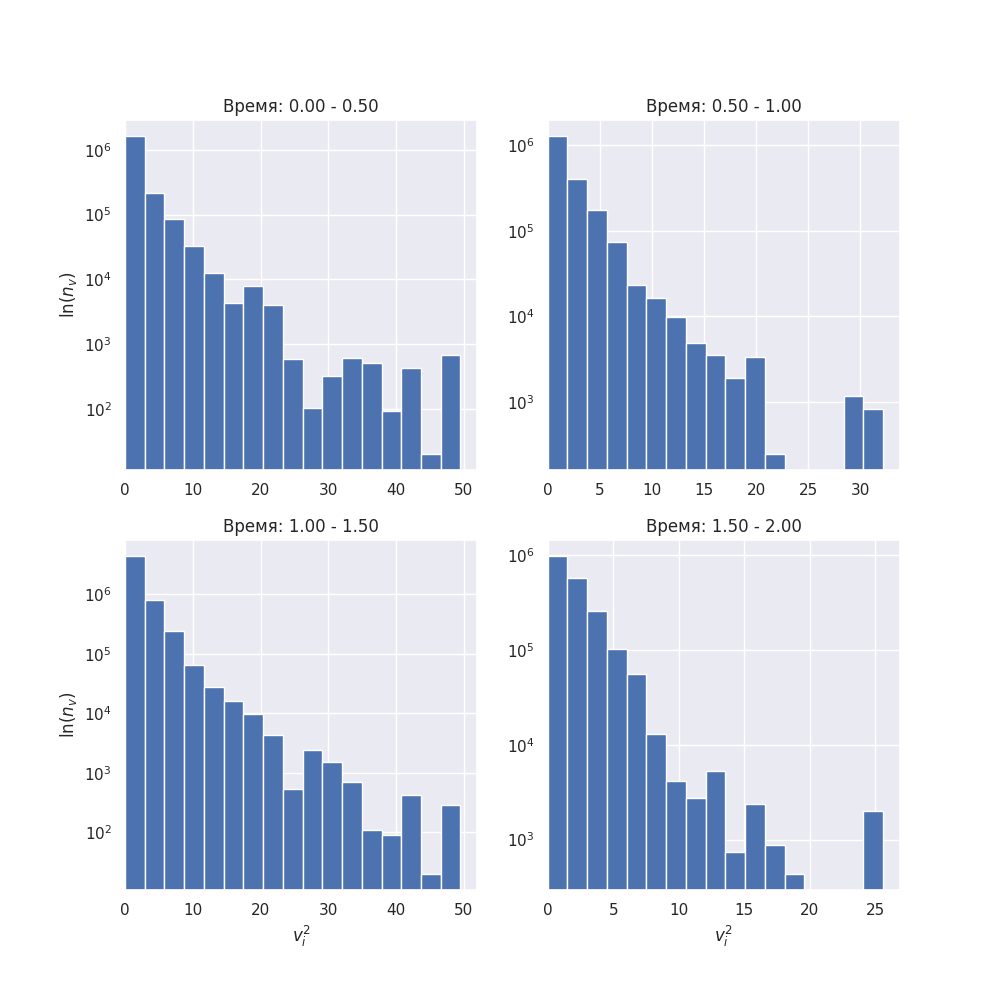
\includegraphics[width=\textwidth]{../../media/velocities1.png}
    % \caption{}
    % \label{fig:}
\end{figure}

\begin{figure}[H]
    \centering
    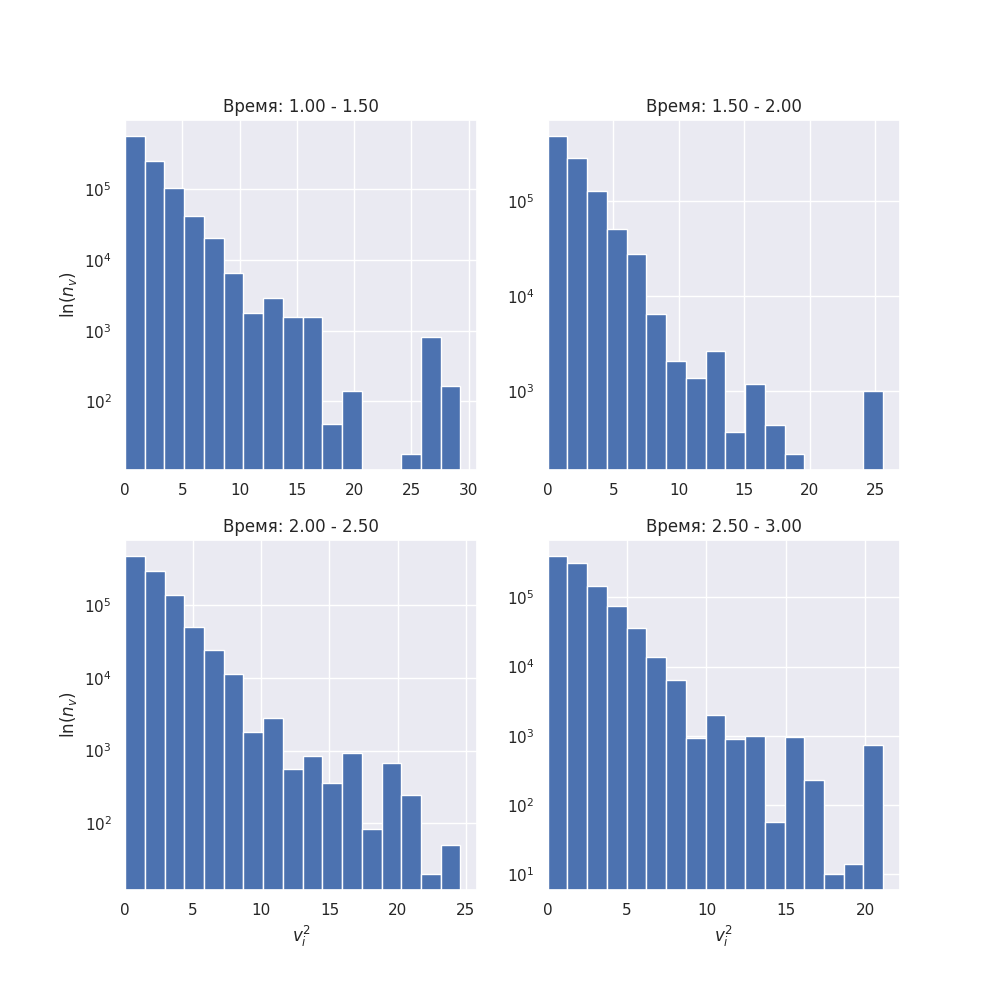
\includegraphics[width=\textwidth]{../../media/velocities2.png}
    % \caption{}
    % \label{fig:}
\end{figure}

\section{Время динамической памяти }

\[
t_m \approx 3
\] 

\begin{equation}
    <\Delta r^2(t)> = \frac{1}{N} \sum_{i = 1}^N (\mathbf{r}_i(t) - \mathbf{r}_i'(t))^2
\end{equation}

\begin{equation}
    <\Delta v^2(t)> = \frac{1}{N} \sum_{i = 1}^N (\mathbf{v}_i(t) - \mathbf{v}_i'(t))^2
\end{equation}

\begin{figure}[H]
    \centering
    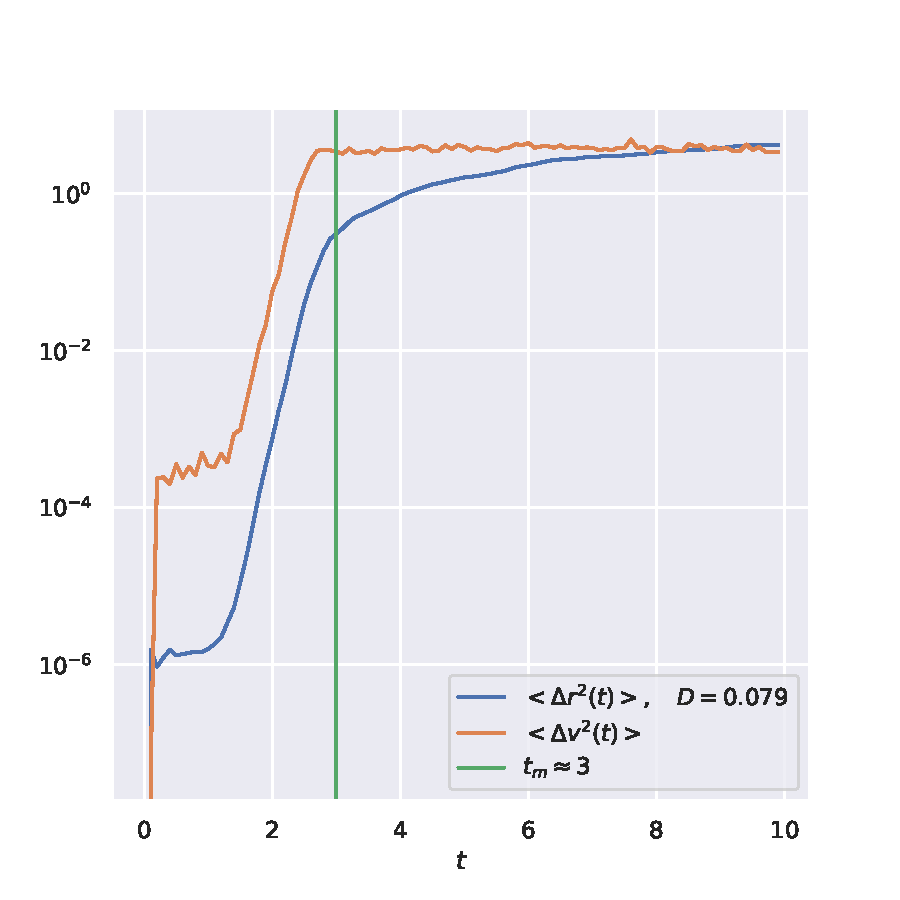
\includegraphics[width=0.8\textwidth]{../../media/tm.pdf}
    \caption{Усреднённые разбегания координат \(<\Delta r^2(t)>\) и скоростей \(<\Delta v^2(t)>\) на двух траекториях, рассчитанных из тождественных начальных условий с шагами \(\Delta t_1 = 0.001\) и \(\Delta t_2 = 0.0001\). Параметры записаны в таблицу \ref{tab1}.}
    % \label{fig:}
\end{figure}

\begin{table}[H]
    \centering
    \caption{Параметры симуляции.}
    \label{tab1}
    \begin{tabular}{| c | c |}
        \hline
        Количество частицы & 64 \\
        \hline
        Шаг по времени 1 & 0.001 \\
        \hline
        Шаг по времени 2 & 0.0001 \\
        \hline
        Температура & 0.44 \\
        \hline
        Плотность & 0.5 \\
        \hline
    \end{tabular}
\end{table}

\section{Уравнеие состояния}

\subsection{Зависимость давления системы от плотности}

\begin{figure}[H]
    \centering
    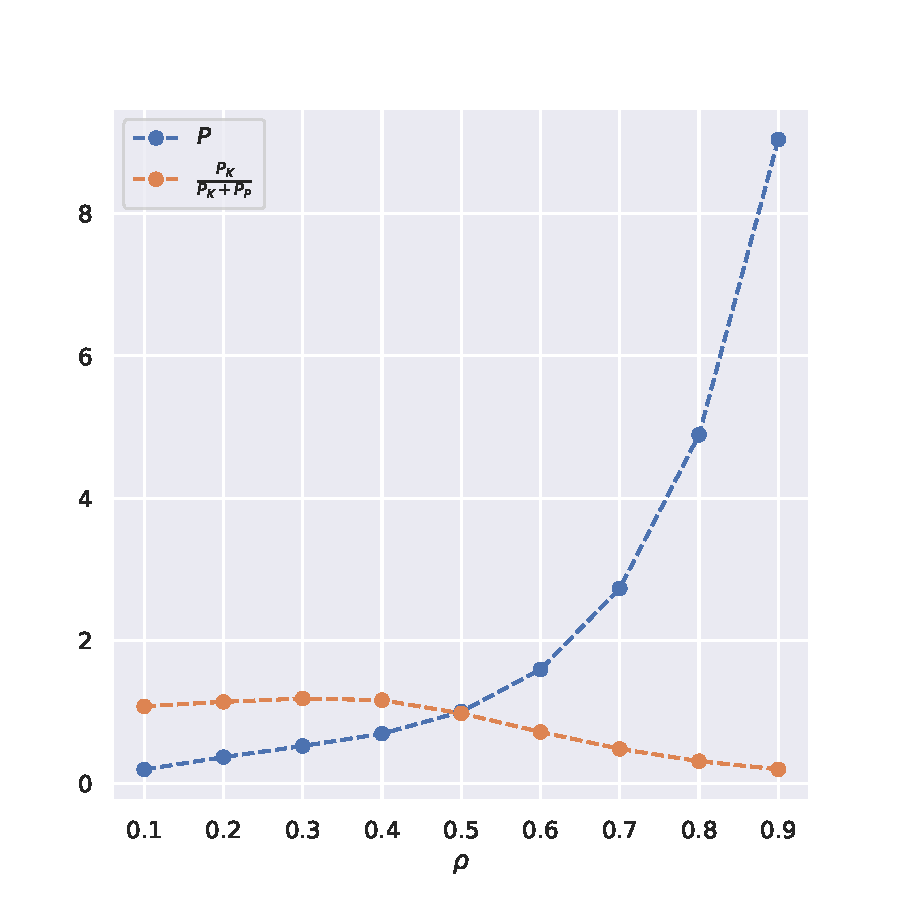
\includegraphics[width=0.8\textwidth]{../../media/pressure.pdf}
\caption{График зависимости давления \(P\) и \(P_k / (P_k + P_P)\) от плотностей, где \(P_k\) - кинетический вклад в давление и \(P_P\) - вириальный вклад. Параметры записаны в таблице \ref{tab2}.}
    \label{fig-eos}
\end{figure}

\subsection{Зависимость сжимаемости системы от плотности}

\begin{figure}[H]
    \centering
    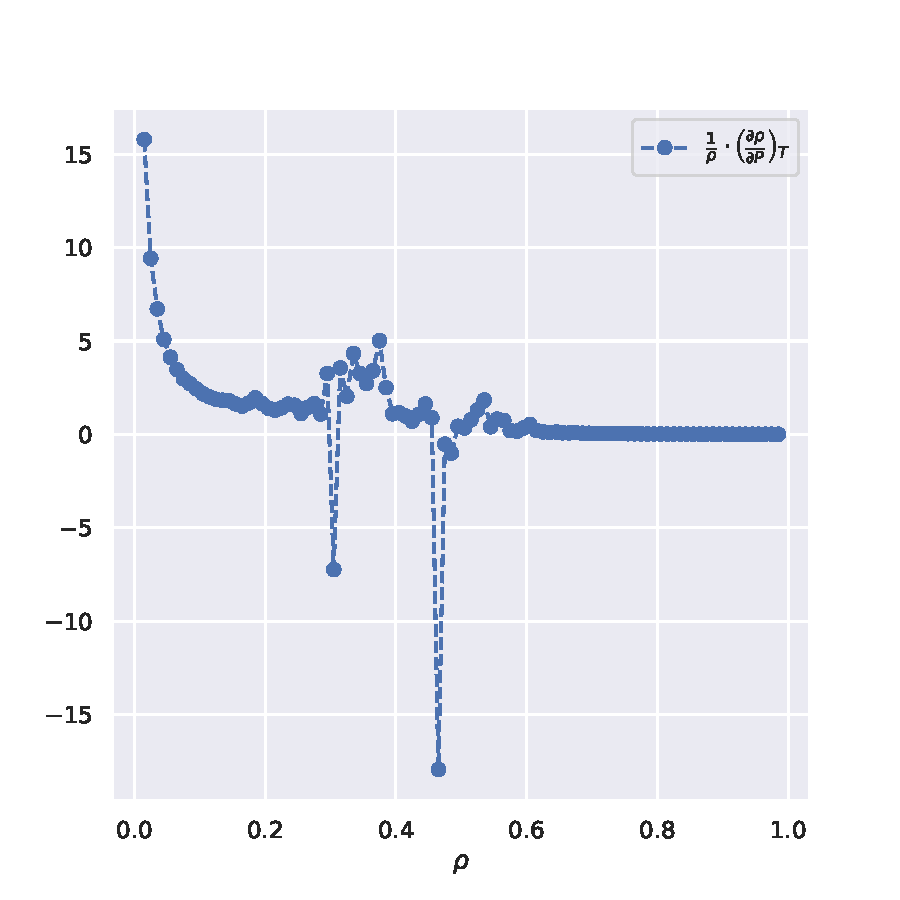
\includegraphics[width=0.8\textwidth]{../../media/compr.pdf}
    \caption{График зависимости сжимаемости от плотности
    \(T = 2\). Параметры записаны в таблице \ref{tab2}.}
    \label{fig-compr}
\end{figure}

\subsection{Проверка формулы для поправки давления 
при обрезке потенциала}

\begin{figure}[H]
    \centering
    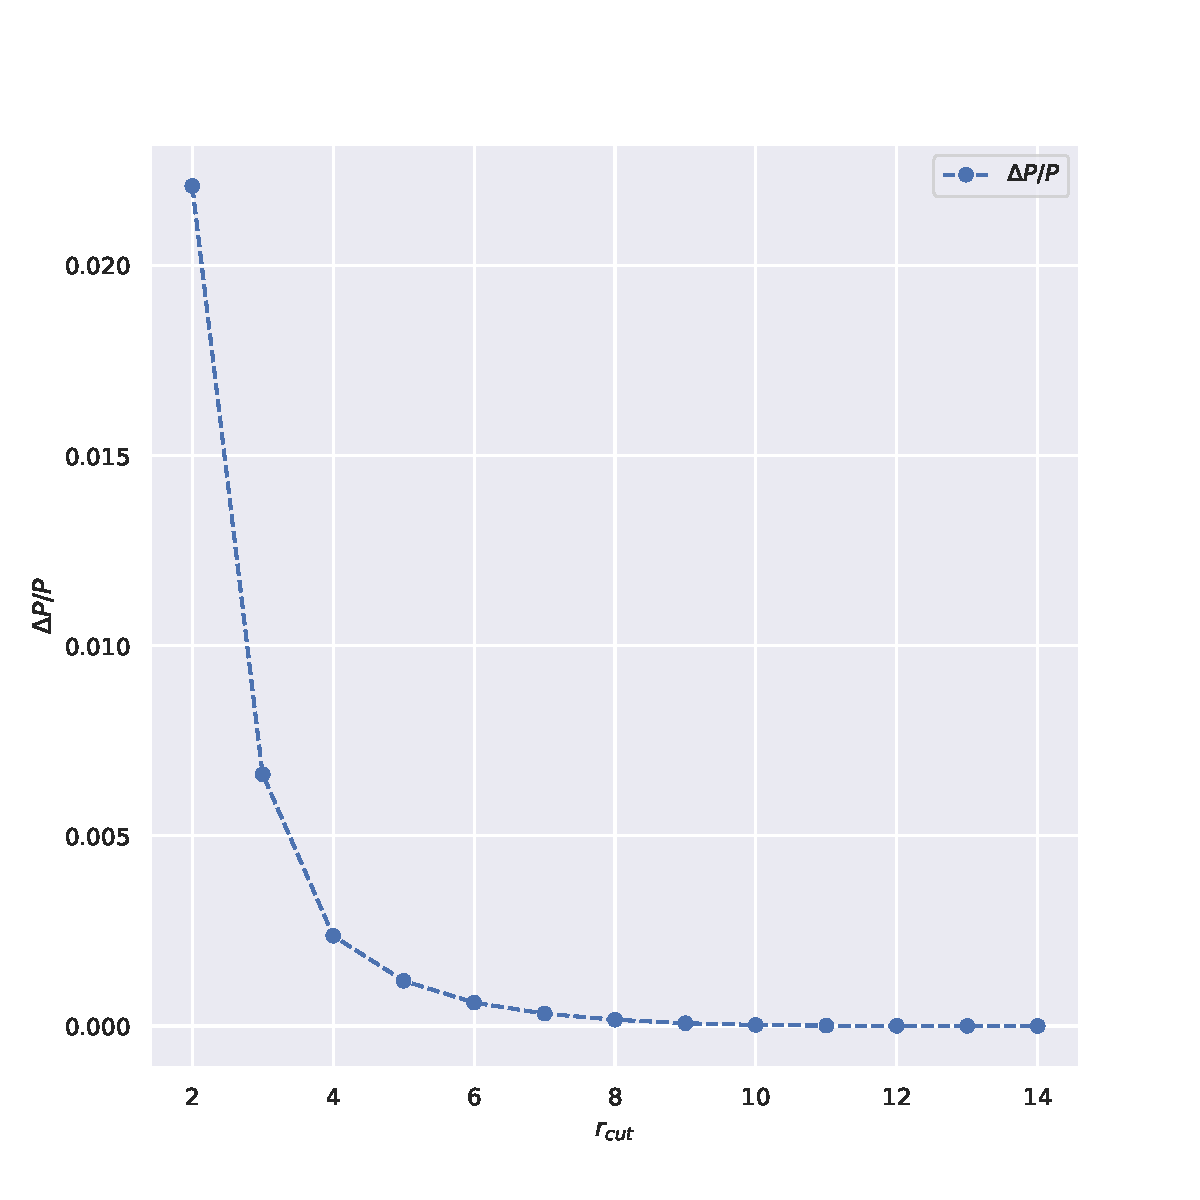
\includegraphics[width=0.8\textwidth]{../../media/rcut.pdf}
    \caption{График зависимости ошибки в давление от обрезки
    потенциала \(r_{cut}\), где \(\Delta P\) - это разность 
между давление полученное без обрезки и давление полученное 
с обрезкой потенциала. 
Параметры записаны в таблице \ref{tab2}.}
    \label{fig-rcut}
\end{figure}

\begin{table}[H]
    \centering
    \caption{Параметры симуляции.}
    \label{tab2}
    \begin{tabular}{| c | c |}
        \hline
        Количество частицы & 512 \\
        \hline
        Шаг по времени & 0.001 \\
        \hline
        Температура & 2 \\
        \hline
        Плотность & 0.1 \\
        \hline
    \end{tabular}
\end{table}

\section{Метод блочных средних}

\begin{figure}[H]
    \centering
    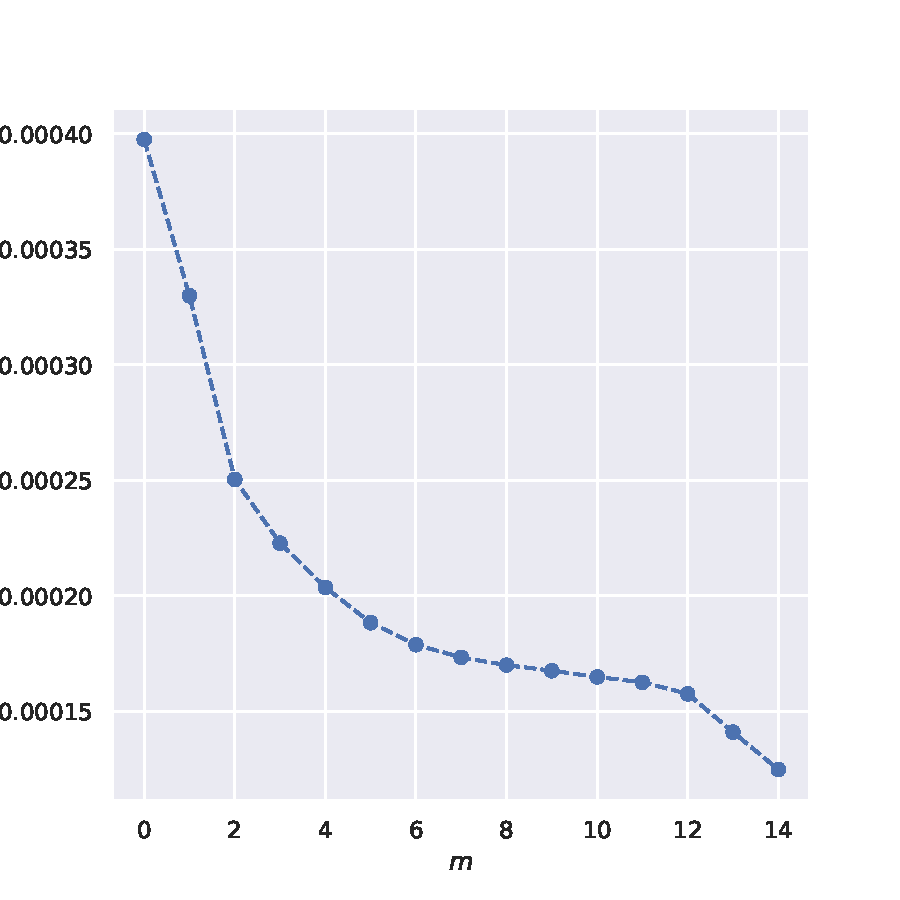
\includegraphics[width=0.8\textwidth]{../../media/blocks.pdf}
    \caption{График зависимости стандартного отклонения полной энергии от количества операций. Параметры записаны в таблице \ref{tab4}.}
    % \label{fig-compr}
\end{figure}

\begin{table}[H]
    \centering
    \caption{Параметры симуляции.}
    \label{tab4}
    \begin{tabular}{| c | c |}
        \hline
        Количество шагов & 1000000 \\
        \hline
        Количество частицы & 64 \\
        \hline
        Шаг по времени & 0.001 \\
        \hline
        Плотность & 0.1 \\
        \hline
    \end{tabular}
\end{table}

\end{document}

